\sectionorchapter{Experimental asymptotics of
\texorpdfstring{$\CatalanNumber a\spc\of{a,b}$}{Ca spc(a,b)}}
\label{appendixExperimental}
Here we examine the exponential asymptotic behaviour of $\CatalanNumber a\spc\of{a,b}$ as a
function of $a+b$; this provides the asymptotics of the bound for
$\gn_{\pointset P}\of{\langle^a\rangle^b\langle^b\rangle^a}$. Specifically, we will be looking
at the behaviour for constant $\gh=\frac{b}{a}$.

The definition (\ref{spcDefinition}) of $\spc$,\begin{equation*}
\spc\of{a,b}\DefineAs
\sum{S\in\binom{[a]}{a-b}} \eggspacing{\quad} \prod{\gc\in\cells\of{[a] \setminus S}}\CatalanNumber {\Cardinality \gc}
\text,
\end{equation*}
has exponentially many terms in the sum for constant $\gh$, so it is highly impractical to compute.

However, using recurrence (\ref{spcRecurrence1}),
\begin{align*}\spc\of{a,b} &= \sum{i=0}[b]
\CatalanNumber {i}
\spc\of{a-i-1,b-i} &\text{for $b<a$,} \\
\spc\of{a,a} &= \CatalanNumber a \text,
\end{align*}
we can use memoization to compute $\spc\of{a,b}$ in cubic time.

We use the following \emph{Mathematica} code:
\begin{verbatim}
spc[a_, a_] := spc[a, a] = CatalanNumber[a];
spc[a_, b_] := spc[a, b] =
  Sum[spc[i, i] spc[a - i - 1, b - i], {i, 0, b}];
\end{verbatim}
Note that we replace the Catalan number $\CatalanNumber i$ in the summands by $\spc\of{i,i}$ in
order to benefit from the memoizatoin of Catalan numbers. While this does not visibly change the
order of the asymptotics for the values of $i$ that we are considering, it improves performance by
a noticeable constant.

This allows us to draw some plots (figure~\ref{figSpcExperimental}) to take an educated guess at
the behaviour of $\CatalanNumber a\spc\of{a,b}$. From this we can conjecture that
$\gn_{\pointset P}\of{\langle^a\rangle^b\langle^b\rangle^a}$ is at most $\BigO\of{5^n}$.

\begin{figure}[htb!]
\centering
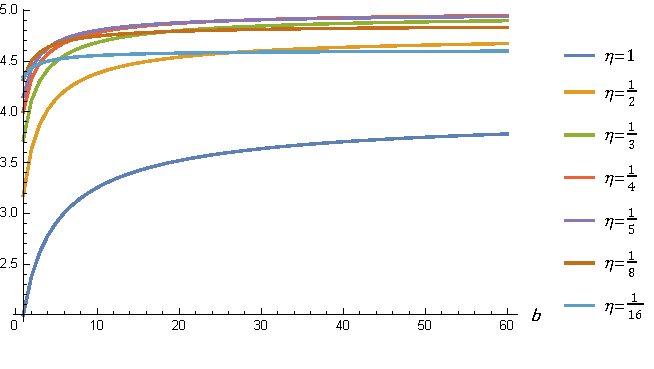
\includegraphics[scale=1]{spc-asymptotics}
\caption{Plots of $\pa{4^{a}\spc\of{a,b}}^{\frac{1}{a+b}}$,
where $a=\frac{b}{\gh}$,
as a fuction of $b$, for various values of $\gh$. As $b$ tends to infinity, this tends to the base
of the exponential bound.
We use $4^a$ rather than $\CatalanNumber a$ because we want to get rid of as many polynomial factors
as possible, since we are looking for the exponential behaviour.
Note that the topmost curve seems to asymptotically approach
$5$.\label{figSpcExperimental}}
\end{figure}

\sectionorchapter{An upper bound for \texorpdfstring{$\spc$}{spc} using the
\texorpdfstring{$\RiemannZeta$}{Zeta} function}
\label{appendixZetaBound}
We can use the recurrence (\ref{spcRecurrence1})
\begin{align*}\spc\of{a,b} &= \sum{i=0}[b]
\CatalanNumber {i}
\spc\of{a-i-1,b-i} &\text{for $b<a$,} \\
\spc\of{a,a} &= \CatalanNumber a \text,
\end{align*}
to derive an exponential bound for $\spc\of{a,b}$ as a function of $a+b$.
We will do so by induction.

We first show an upper bound on the Catalan numbers which we will use in the induction.
\begin{remark}
For $a\geq 1$, we have\begin{equation}
\CatalanNumber a \leq \frac{4^a}{a^{\frac 3 2}\sqrt{\Pi}}-\pa{4\frac {\sqrt 2} {\sqrt \Pi}-2} \text.\label{CatalanZetaFriendlyBound}
\end{equation}
\begin{proof}
We use the upper bound shown by R.~D.~Dutton and R.~C.~Brigham in \cite{DuttonBrigham1986},\[
\CatalanNumber a\leq \frac{4^a}{\pa{a+1}\sqrt{a\Pi}}\text.
\]
It follows that\[
\frac{4^a}{a^{\frac 3 2}\sqrt{\Pi}} - \CatalanNumber a \geq \frac{4^a}{a^{\frac 3 2}\sqrt{\Pi}} - \frac{4^a}{\pa{a+1}\sqrt{a\Pi}} = \frac{4^a}{a^{\frac 3 2}\pa{a+1}\sqrt{\Pi}}\text,
\]
which is an increasing function of $a$ for $a>2$. For $n=3$, we have\[
\frac{4^a}{a^{\frac 3 2}\pa{a+1}\sqrt{\Pi}}=\frac{16}{3\sqrt{3\Pi}}>4\frac {\sqrt 2} {\sqrt \Pi}-2\text.
\]
There thus remains to check (\ref{CatalanZetaFriendlyBound}) for $n=1$ and $n=2$. It holds for both, with equality at $n=2$.
\end{proof}
\end{remark}
We now go back to bounding $\spc\of{a,b}$.
Let $b<a$. Define\[
\gcq\DefineAs 1+\frac{\RiemannZeta\of{\frac 3 2}}{\sqrt{\Pi}}-\frac{1}{3}\pa{4\frac {\sqrt 2} {\sqrt \Pi}-2}\text,
\]
and observe that $\gcq\approx 2.0767 > 2$. The reason for this definition will become clear at the end of the calculation.
Assuming that for all $\spc\of{a',b'}$ involved in the sum
for $\spc\of{a,b}$,\[
\spc\of{a',b'}\leq\gcq^{a'+b'}\text,
\]
we get\begin{align*}
\spc\of{a,b} &= \sum{i=0}[b] \CatalanNumber {i} \spc\of{a-i-1,b-i} \\
 &\leq \sum{i=0}[b] \CatalanNumber {i} \gcq^{a+b-2i-1} \\
 &= \gcq^{a+b-1}\pa{1+\sum{i=1}[b] \CatalanNumber {i} \gcq^{-2i}}\\
\intertext{using (\ref{CatalanZetaFriendlyBound}),}
 &\leq \gcq^{a+b-1}\pa{1+\sum{i=1}[b] \pa{\frac{4^i}{i^{\frac 3 2}\sqrt{\Pi}}-\pa{4\frac {\sqrt 2} {\sqrt \Pi}-2}} \gcq^{-2i}} \\
\intertext{with $\gcq > 2$,}
 &\leq \gcq^{a+b-1}\pa{1+\sum{i=1}[b] \pa{\frac{4^i}{i^{\frac 3 2}\sqrt{\Pi}}-\pa{4\frac {\sqrt 2} {\sqrt \Pi}-2}} 4^{-i}} \\
 &= \gcq^{a+b-1}\pa{1+\sum{i=1}[b] \pa{\frac{1}{i^{\frac 3 2}\sqrt{\Pi}}-\pa{4\frac {\sqrt 2} {\sqrt \Pi}-2} 4^{-i}}} \\
 &\leq \gcq^{a+b-1}\pa{1+\sum{i=1}[\infty] \pa{\frac{1}{i^{\frac 3 2}\sqrt{\Pi}}-\pa{4\frac {\sqrt 2} {\sqrt \Pi}-2} 4^{-i}}} \\
 &= \gcq^{a+b-1}\pa{1+\frac{\RiemannZeta\of{\frac 3 2}}{\sqrt{\Pi}}-\frac{1}{3}\pa{4\frac {\sqrt 2} {\sqrt \Pi}-2}} \\
 &= \gcq^{a+b}\text.
\end{align*}
We start the induction for $a=b$ with $\spc\of{a,a}=\CatalanNumber a \leq 4^{a} < \gcq^{a+a}$.
This gives us the bound\[
\spc\of{a,b}\leq\gcq^{a+b}\text,
\]
and so, with $\gh=\frac{b}{a}$,\begin{equation}
\gn_{\pointset P}\of{\langle^a\rangle^b\langle^b\rangle^a} \leq \pa{\CatalanNumber a \spc\of{a,b}}^2\leq \pa{4^{\frac{1}{\gh+1}} \gcq}^{n}\text.
\label{zetaBound}
\end{equation}
A plot of that bound is shown in figure~\ref{figZetaBound}.

\begin{figure}[htb!]
\centering
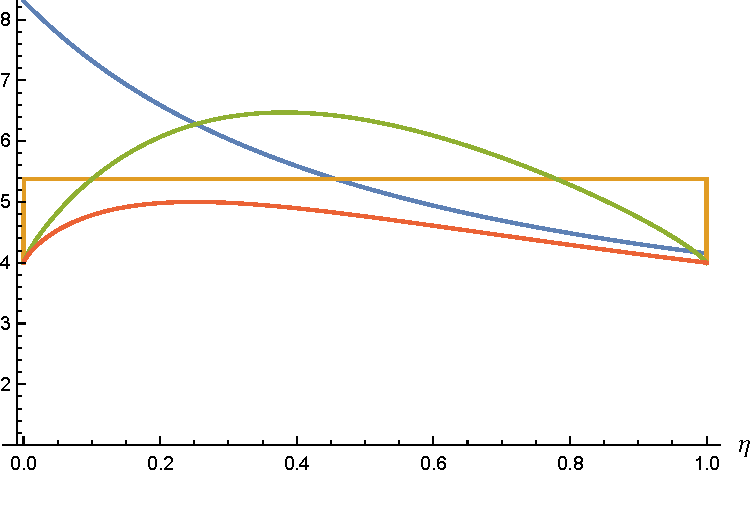
\includegraphics[scale=0.75]{spc-zeta-bound.pdf}
\caption{Blue: the base of the exponential bound (\ref{zetaBound}) as a function of $\gh$. Yellow: pre-existing bounds.
Green: the bound (\ref{binomialBound}), for comparison. Red: the actual asymptotics of $\CatalanNumber a \spc\of{a,b}$.\label{figZetaBound}}
\end{figure}